% =========================================================
% Bounds, Suprema, Infima + Table + Figure
% =========================================================

\subsection{Bounds and Extremal Values}

% ---------------------------------------------------------
% Toolkit
% ---------------------------------------------------------
\begin{tcolorbox}[colback=gray!6, colframe=gray!40, arc=2pt,
  left=6pt, right=6pt, top=4pt, bottom=4pt,
  title={\small\textbf{Bounds Extremal Values — Quick Reference}},
  fonttitle=\small\bfseries]
\begin{tabular}{@{}p{0.28\textwidth}p{0.68\textwidth}@{}}
\textbf{Core items} & Key definitions/results introduced in this file.\\
\textbf{How to use} & Read the boxed items first; proofs and consequences follow.\\
\textbf{Dependencies} & Refer back to earlier sections as needed.\\
\end{tabular}
\end{tcolorbox}


\begin{remark}[Predicate vs.\ Existence: Structural Template]
Each bound-type concept (maximum, minimum, upper bound, supremum, etc.)
is defined by a predicate on $\mathbb{R}$. Given $A \subseteq \mathbb{R}$,
let $P_A(x)$ denote such a predicate.

\medskip
\textbf{Predicate form.}
The statement ``$x$ is a $P$-object of $A$'' means $P_A(x)$ holds for a
specific, identified element $x \in \mathbb{R}$. To prove this, one
exhibits the element and verifies each condition in $P_A(x)$.

\medskip
\textbf{Existence form.}
The statement ``$A$ has a $P$-object'' means $\exists x\; P_A(x)$.
Once established, one may fix such an $x$ and reason about it
(existential instantiation).

\medskip
\textbf{Notational glosses.}
\begin{itemize}
  \item ``$x$ is a $P$-object of $A$'' abbreviates $P_A(x)$.
  \item ``$A$ has a $P$-object'' abbreviates $\exists x\; P_A(x)$.
\end{itemize}

\medskip
\textbf{Proof strategy summary.}
\begin{table}[h]
\centering
\renewcommand{\arraystretch}{1.4}
\begin{tabular}{@{} p{4cm} p{3cm} p{6cm} @{}}
\toprule
\textbf{Goal} & \textbf{Form} & \textbf{Strategy} \\
\midrule
$P_A(x)$ & Predicate & Exhibit $x$; verify $P_A(x)$ directly. \\
\addlinespace[0.3em]
$\exists x\; P_A(x)$ & Existence & Construct or name a candidate; verify $P_A(x)$. \\
\midrule
\textit{Hypothesis:} $\exists x\; P_A(x)$ & --- & Fix such an $x$; use $P_A(x)$ in further reasoning. \\
\bottomrule
\end{tabular}
\caption*{\footnotesize The hypothesis row reflects existential instantiation,
not a proof goal.}
\end{table}
\end{remark}

\begin{figure}[h]
    \centering
    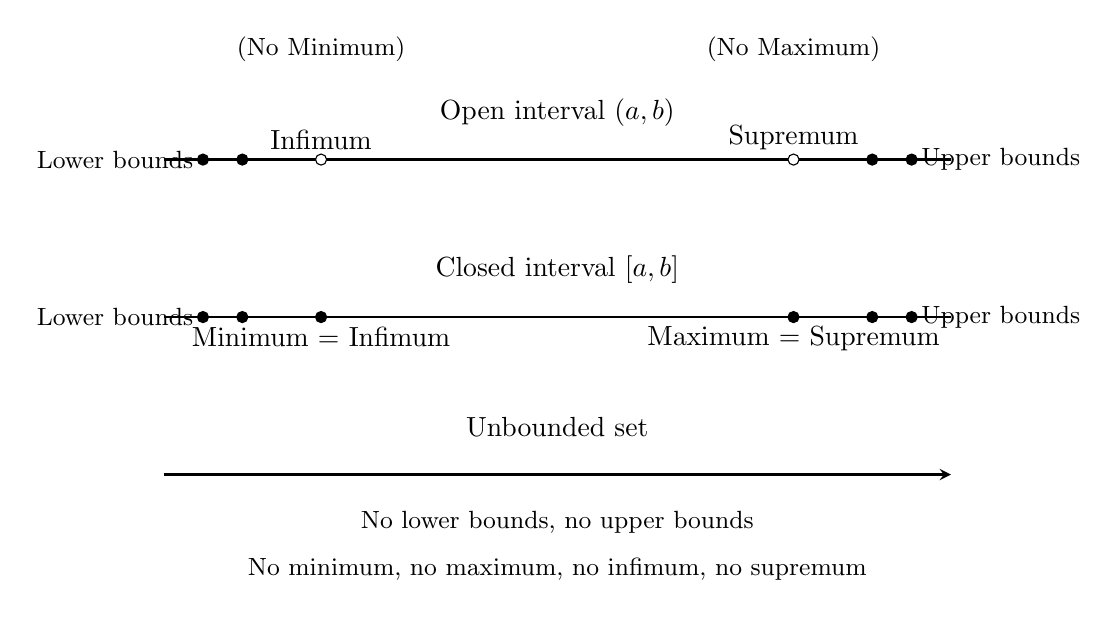
\begin{tikzpicture}[x=1cm,y=1cm,>=stealth]

% =====================
% OPEN INTERVAL (a,b)
% =====================
\draw[thick] (-5,3) -- (5,3);
\draw[fill=white] (-3,3) circle (2pt);
\draw[fill=white] (3,3) circle (2pt);

\node at (0,3.6) {Open interval $(a,b)$};

% Infimum / Supremum
\node[above] at (-3,3) {Infimum};
\node[above] at (3,3) {Supremum};
\node at (-3,4.4) {\small (No Minimum)};
\node at (3,4.4) {\small (No Maximum)};

% Lower bounds
\draw[fill] (-4.5,3) circle (2pt);
\draw[fill] (-4,3) circle (2pt);
\node[left] at (-4.5,3) {\small Lower bounds};

% Upper bounds
\draw[fill] (4,3) circle (2pt);
\draw[fill] (4.5,3) circle (2pt);
\node[right] at (4.5,3) {\small Upper bounds};

% =====================
% CLOSED INTERVAL [a,b]
% =====================
\draw[thick] (-5,1) -- (5,1);
\draw[fill] (-3,1) circle (2pt);
\draw[fill] (3,1) circle (2pt);

\node at (0,1.6) {Closed interval $[a,b]$};

% Min / Max
\node[below] at (-3,1) {Minimum = Infimum};
\node[below] at (3,1) {Maximum = Supremum};

% Lower bounds
\draw[fill] (-4.5,1) circle (2pt);
\draw[fill] (-4,1) circle (2pt);
\node[left] at (-4.5,1) {\small Lower bounds};

% Upper bounds
\draw[fill] (4,1) circle (2pt);
\draw[fill] (4.5,1) circle (2pt);
\node[right] at (4.5,1) {\small Upper bounds};

% =====================
% UNBOUNDED SET
% =====================
\draw[thick,->] (-5,-1) -- (5,-1);

\node at (0,-0.4) {Unbounded set};

\node at (0,-1.6)
{\small No lower bounds, no upper bounds};

\node at (0,-2.2)
{\small No minimum, no maximum, no infimum, no supremum};
\end{tikzpicture}
    \caption{Bounds, Extrema, Infimum, and Supremum for Subsets of $\mathbb{R}$.}
    \label{fig:bounds-extrema}
\end{figure}

% ---------------------------------------------------------
% Summary table: predicate and existence forms
% ---------------------------------------------------------
\begin{table}[h]
\centering
\renewcommand{\arraystretch}{1.6}
\begin{tabular}{@{} p{2.2cm} p{5.8cm} p{3.2cm} p{3.2cm} @{}}
\toprule
\textbf{Concept} & \textbf{Predicate} $P_A(x)$ & \textbf{Predicate Form} & \textbf{Existence Form} \\
\midrule
Upper bound
  & $\forall a \in A,\ a \leq x$
  & $x$ is an upper bound of $A$
  & $A$ is bounded above \\
\addlinespace[0.2em]
Lower bound
  & $\forall a \in A,\ a \geq x$
  & $x$ is a lower bound of $A$
  & $A$ is bounded below \\
\midrule
Maximum
  & $x \in A \;\land\; \forall a \in A,\ a \leq x$
  & $x = \max A$
  & $A$ has a maximum \\
\addlinespace[0.2em]
Minimum
  & $x \in A \;\land\; \forall a \in A,\ a \geq x$
  & $x = \min A$
  & $A$ has a minimum \\
\midrule
Supremum
  & $(\forall a \in A,\ a \leq x)$
    $\land\; (\forall \varepsilon > 0,\ \exists a \in A,\ a > x - \varepsilon)$
  & $x = \sup A$
  & $\sup A$ exists \\
\addlinespace[0.2em]
Infimum
  & $(\forall a \in A,\ a \geq x)$
    $\land\; (\forall \varepsilon > 0,\ \exists a \in A,\ a < x + \varepsilon)$
  & $x = \inf A$
  & $\inf A$ exists \\
\bottomrule
\end{tabular}
\caption*{\footnotesize
  Rows are grouped by logical complexity: bounds (universal only),
  extrema (membership $+$ universal), least/greatest bounds
  (universal $+$ approximation).
  The predicate column gives the condition that must hold for a
  specific $x \in \mathbb{R}$; the existence form asserts $\exists x\; P_A(x)$.}
\end{table}

% ---------------------------------------------------------
% Definitions: bounds first, then extrema, then sup/inf
% (ordered by logical dependency and increasing complexity)
% ---------------------------------------------------------

\begin{tcolorbox}[colback=propbox, colframe=propborder, arc=2pt,
  left=6pt, right=6pt, top=4pt, bottom=4pt,
  title={\small\textbf{Definition (Upper Bound)}},
  fonttitle=\small\bfseries]
Let $A \subseteq \mathbb{R}$.
A number $u \in \mathbb{R}$ is an \emph{upper bound} for $A$ if
\[
\forall a \in A,\quad a \le u.
\]
\end{tcolorbox}

\begin{tcolorbox}[colback=propbox, colframe=propborder, arc=2pt,
  left=6pt, right=6pt, top=4pt, bottom=4pt,
  title={\small\textbf{Definition (Lower Bound)}},
  fonttitle=\small\bfseries]
Let $A \subseteq \mathbb{R}$.
A number $\ell \in \mathbb{R}$ is a \emph{lower bound} for $A$ if
\[
\forall a \in A,\quad \ell \le a.
\]
\end{tcolorbox}

\begin{tcolorbox}[colback=propbox, colframe=propborder, arc=2pt,
  left=6pt, right=6pt, top=4pt, bottom=4pt,
  title={\small\textbf{Definition (Bounded Above / Below)}},
  fonttitle=\small\bfseries]
A set $A \subseteq \mathbb{R}$ is said to be:
\begin{itemize}
  \item \emph{bounded above} if it has at least one upper bound;
  \item \emph{bounded below} if it has at least one lower bound;
  \item \emph{bounded} if it is both bounded above and bounded below.
\end{itemize}
\end{tcolorbox}

\begin{tcolorbox}[colback=propbox, colframe=propborder, arc=2pt,
  left=6pt, right=6pt, top=4pt, bottom=4pt,
  title={\small\textbf{Definition (Maximum)}},
  fonttitle=\small\bfseries]
Let $A \subseteq \mathbb{R}$.
A number $m \in A$ is a \emph{maximum} of $A$, written $m = \max A$, if
\[
\forall a \in A,\quad a \le m.
\]
\end{tcolorbox}

\begin{tcolorbox}[colback=propbox, colframe=propborder, arc=2pt,
  left=6pt, right=6pt, top=4pt, bottom=4pt,
  title={\small\textbf{Definition (Minimum)}},
  fonttitle=\small\bfseries]
Let $A \subseteq \mathbb{R}$.
A number $m \in A$ is a \emph{minimum} of $A$, written $m = \min A$, if
\[
\forall a \in A,\quad m \le a.
\]
\end{tcolorbox}

\begin{remark}
Every maximum is an upper bound that is also a member of $A$; every
minimum is a lower bound that is also a member of $A$.
In particular, $\max A$ and $\min A$ need not exist, but when they do
they are unique.
The concepts of supremum and infimum generalise this: they are the
\emph{least} upper bound and \emph{greatest} lower bound respectively,
and need not belong to $A$. Both are unique when they exist
(see Proposition~\ref{prop:sup-unique}).
\end{remark}

\begin{proposition}[Uniqueness of Supremum and Infimum]
\label{prop:sup-unique}
Let $A \subseteq \mathbb{R}$ be nonempty.
If $\sup A$ exists, it is unique. If $\inf A$ exists, it is unique.
\end{proposition}

\begin{proof}
We prove uniqueness of the supremum; the argument for the infimum is
symmetric. Suppose $s$ and $s'$ both satisfy the definition of $\sup A$.
Since $s = \sup A$ and $s'$ is an upper bound for $A$, we have $s \le s'$.
Since $s' = \sup A$ and $s$ is an upper bound for $A$, we have $s' \le s$.
Hence $s = s'$.
\end{proof}

\begin{tcolorbox}[colback=propbox, colframe=propborder, arc=2pt,
  left=6pt, right=6pt, top=4pt, bottom=4pt,
  title={\small\textbf{Definition (Supremum (Least Upper Bound))}},
  fonttitle=\small\bfseries]
Let $A \subseteq \mathbb{R}$ be nonempty and bounded above.
A number $s \in \mathbb{R}$ is the \emph{supremum} of $A$,
written $s = \sup A$, if:
\begin{enumerate}
  \item $s$ is an upper bound for $A$, and
  \item if $u$ is any upper bound for $A$, then $s \le u$.
\end{enumerate}
\end{tcolorbox}

\begin{tcolorbox}[colback=propbox, colframe=propborder, arc=2pt,
  left=6pt, right=6pt, top=4pt, bottom=4pt,
  title={\small\textbf{Definition (Infimum (Greatest Lower Bound))}},
  fonttitle=\small\bfseries]
Let $A \subseteq \mathbb{R}$ be nonempty and bounded below.
A number $s \in \mathbb{R}$ is the \emph{infimum} of $A$,
written $s = \inf A$, if:
\begin{enumerate}
  \item $s$ is a lower bound for $A$, and
  \item if $\ell$ is any lower bound for $A$, then $\ell \le s$.
\end{enumerate}
\end{tcolorbox}

% ---------------------------------------------------------
% Equivalent formulations of supremum and infimum.
% ---------------------------------------------------------

\subsubsection{Equivalent Formulations}

The definition of supremum requires checking all upper bounds. The
following proposition gives an equivalent condition that is often easier
to apply in practice, replacing the universal quantifier over upper bounds
with a local $\varepsilon$-witness condition.

\begin{proposition}[$\varepsilon$-Characterization of Supremum and Infimum]
\label{prop:eps-char}
Let $A \subseteq \mathbb{R}$ be nonempty. Both of the following hold.
\begin{enumerate}
  \item If $A$ is bounded above and $s \in \mathbb{R}$, then $s = \sup A$
        if and only if both of the following conditions hold:
        \begin{enumerate}[(a)]
          \item $s$ is an upper bound for $A$, and
          \item for every $\varepsilon > 0$, there exists $a \in A$ such that
                $s - \varepsilon < a$.
        \end{enumerate}
  \item If $A$ is bounded below and $s \in \mathbb{R}$, then $s = \inf A$
        if and only if both of the following conditions hold:
        \begin{enumerate}[(a)]
          \item $s$ is a lower bound for $A$, and
          \item for every $\varepsilon > 0$, there exists $a \in A$ such that
                $a < s + \varepsilon$.
        \end{enumerate}
\end{enumerate}
\end{proposition}

\begin{proof}
We prove (1); the proof of (2) is symmetric.

($\Rightarrow$) Suppose $s = \sup A$. Then $s$ is an upper bound by
definition. Let $\varepsilon > 0$. Since $s - \varepsilon < s$ and $s$ is
the \emph{least} upper bound, $s - \varepsilon$ is not an upper bound for
$A$. Hence there exists $a \in A$ with $a > s - \varepsilon$.

($\Leftarrow$) Suppose (a) and (b) hold. Let $u$ be any upper bound for
$A$. Suppose for contradiction that $u < s$. Set $\varepsilon = s - u > 0$.
By (b), there exists $a \in A$ with $a > s - \varepsilon = u$, contradicting
$u$ being an upper bound. Hence $s \le u$, so $s$ is the least upper bound.
\end{proof}

\begin{corollary}[$\varepsilon$-Approximation]
\label{cor:eps-approx}
Let $A \subseteq \mathbb{R}$ be nonempty.
\begin{enumerate}
  \item If $s = \sup A$, then
        $\forall \varepsilon > 0,\ \exists a \in A$ such that
        $s - \varepsilon < a \le s$.
  \item If $s = \inf A$, then
        $\forall \varepsilon > 0,\ \exists a \in A$ such that
        $s \le a < s + \varepsilon$.
\end{enumerate}
\end{corollary}

\begin{proof}
We prove (1); the proof of (2) is symmetric. By
Proposition~\ref{prop:eps-char}(1), there exists $a \in A$ with
$a > s - \varepsilon$. Since $s$ is an upper bound for $A$, we also have
$a \le s$. Hence $s - \varepsilon < a \le s$.
\end{proof}